\chapter{NodeJS}\label{chap:nodejs}
\section{Sarrera}
Node.js\index{Node.js} plataformarekin JavaScript aplikazioak zerbitzarian programatu ahal izango ditugu. Orain arte HTML5ek eskaintzen dituen APIekin egin dugun guztia bezero aldean izan da. Baina web aplikazio batek, orokorrean, bezeroa eta zerbitzari bat behar ditu. Zerbitzariaren aldean programatzeko hainbat aukera ditugu: PHP, ASP.NET, Ruby, Python... eta JavaScript. Azken lengoaia horretan zerbitzarian sortuko ditugun aplikazioak programatzeko, NodeJS (askotan node izenaz laburbilduta) erabiliko dugu. Node Google Chrome-k eskaintzen duen \mbox{JavaScript} motorrean (v8 deritzona) dago oinarrituta. Gaur egun milaka aplikazio daude Node-n programatuta, eta haren inguruan sortu den ekosistema sekulakoa da.

Liburu honetan ez dugu asko sakonduko Node-n (azken finean HTML5en inguruko liburu bat da!), baina gutxienez planteatutako ariketa batzuk egin ahal izateko, gainetik ezagutu behar dugu nola sortu eta nola erabili Node-n egindako aplikazio bat. 

Adibide sinple batekin hasiko gara: betiko \textit{``Hello World''} edo \textit{``Kaixo mundua''} inprimatzen duen HTTP zerbitzari bat programatuko dugu, 4 lerrotan. Hasteko, sortu \hl{zerbitzaria.js} izeneko fitxategia, honako edukiarekin:

\index{http}\index{createServer}\index{response}\index{request}
\begin{lstlisting}[language=javascript]
const http = require('http');
http.createServer (function (request, response) {
	response.writeHead(200, {'Content-Type': 'text/plain'});
	response.end('Kaixo Mundua\n');
}).listen(8000);

console.log('Zerbitzaria http://127.0.0.1:8000/ eskuragarri duzu');
\end{lstlisting}

Lehenengo lerroan \textit{http} modulua kargatzen dugu \textit{require} \index{require} aginduaren bidez. \textit{http} moduluak HTTP zerbitzari bat sortzeko aukera ematen du (2. lerroan), 8000 portuan entzuten jarriko dena. Eskaera (\textit{request}) bat jasotzean  HTTP/200 kodearekin erantzungo du, ``Kaixo Mundua'' edukia bidaliz. Azkenengo lerroak zerbitzariko kontsolan mezu bat pantailaratuko du, informazio gisa.

Martxan jartzeko honako komandoa landuko dugu:

\begin{lstlisting}[language=Bash,numbers=none]
   node zerbitzaria.js
\end{lstlisting}



\begin{figure}[ht]
	\centering
\begin{tikzpicture}[framed]
\node[anchor=south west,inner sep=0] (image) at (0,0)
   {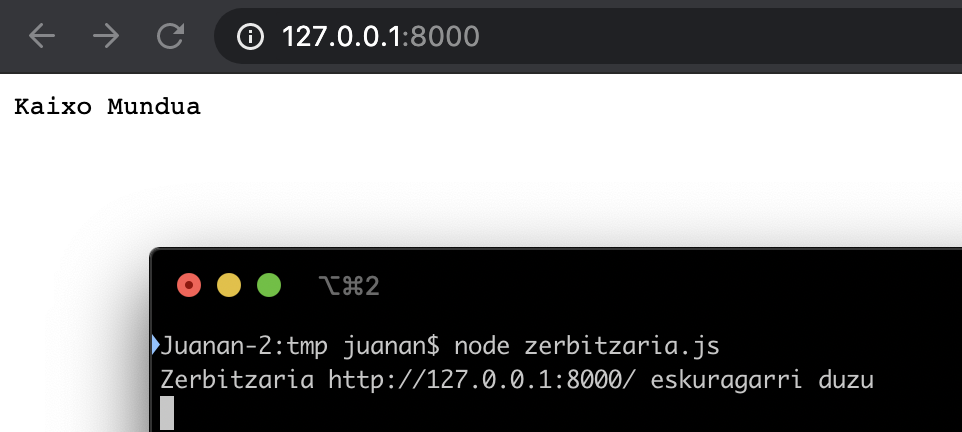
\includegraphics[trim=0cm 0cm 0cm 0cm, clip=true, width=0.75\textwidth]{img/nodezerbitzaria.png}};
\end{tikzpicture}
\caption{Node-n egindako HTTP zerbitzari soil bat.}
\label{fig:node1}
\end{figure}

Prestatu dugun HTTP zerbitzaria gure probatxoak egiteko ondo dago, baina ezin dugu programatu JavaScript lerro bat eskaera mota bakoitzeko! Ziur asko, hasieran jada HTML, JS, CSS eta irudiak prestatuta izango ditugu karpeta batean eta horiek HTTP bidez eskaini nahiko ditugu, ezer programatu gabe. Horretarako (fitxategi estatikoak eskaintzeko), node-k \textit{serve} \index{serve} izeneko HTTP zerbitzari sinple bat eskaintzen du, \textit{npm} pakete-kudeatzailearekin instalatu behar dena. npm (\textit{node package manager}) node-rako paketeak kudeatzeko sistema bat da. Haren erabilera erraza demostratzeko, ikus dezagun nola instala dezakegun \hl{serve} paketea npm-aren bidez.

\begin{alertinfo}{Nondik deskargatu node?}
  NodeJS bere webgune ofizialetik jaits dezakegu (\href{https://nodejs.org}{https://nodejs.org}), Linux, MacOS edo Windows-erako.
\end{alertinfo}

Hasteko, lehenengo komandoa \hl{npm init}\index{npm.init} izango da. Horrekin, mendekotasunak dituen node proiektu berri bat prestatuko dugu. npm init prozesuak galdera asko egiten badu ere, hasieran guztiei \textit{Enter} tekla sakatuz erantzungo diegu. Prozesua bukatzean \hl{package.json} izeneko fitxategi bat sortuko da. Bertan, npm-ak gure aplikaziorako beharrezkoak diren mendekotasunak apuntatuko ditu.

Ondoren, \hl{serve} paketea instalatzeko, \hl{npm install serve}\index{serve} idatziko dugu. Ohart zaitez nola sortzen den \textit{node\_modules}\index{node\_modules} izeneko karpeta bat. Horren barruan \textit{serve} zerbitzariak dituen mendekotasun guztiak instalatu dira automatikoki.

Jarraian, \hl{public/} izeneko karpeta bat sortuko dugu eta bertan HTML orri bat (adibidez, index.html, bertan ``Kaixo mundua!'' idazten duena, berriro ere) sartuko dugu.

Dena prest \textit{serve} zerbitzaria martxan jartzeko!:

\begin{lstlisting}[language=Bash,numbers=none]
serve ./public     
\end{lstlisting}

\begin{figure}[ht]
	\centering
\begin{tikzpicture}
\node[anchor=south west,inner sep=0] (image) at (0,0)
   {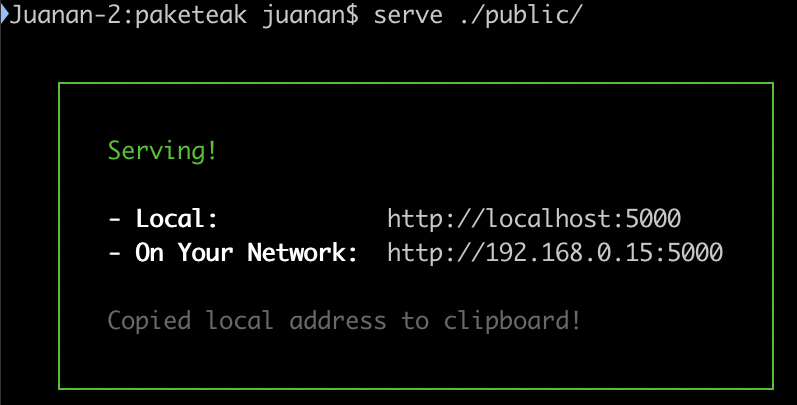
\includegraphics[trim=0cm 0cm 0cm 0cm, clip=true, width=0.75\textwidth]{img/nodeserve.png}};
\end{tikzpicture}
\caption{\textit{Serve} paketearen laguntzaz web zerbitzari oso bat presta dezakegu, (adibidean) 5000 portuan entzuten, lerro bakar batekin: \hl{serve ./public}.}
\label{fig:node2}
\end{figure}

Zerbitzaria modu erosoan martxan jarri ahal izateko, npm komando sinple bat presta dezakegu. Lortu nahi duguna zera da,  \hl{npm start} idaztean, automatikoki \hl{serve ./public} exekutatzea. Horretarako, \textit{package.json} fitxategia \index{package.json} editatuko dugu, zehazki \textit{scripts} atala, honela gera dadin:

\begin{lstlisting}[language=JavaScript,numbers=none]
 {
  "name": "paketeak",
  "version": "1.0.0",
  "description": "",
  "main": "index.js",
  "scripts": {
    "start": "serve ./public",
    "test": "echo \"Error: no test specified\" && exit 1"
  },
  "author": "",
  "license": "ISC",
  "dependencies": {
    "serve": "^11.3.0"
  }
}
\end{lstlisting}

\begin{alertinfo}{npm : node package manager}
  \href{https://www.npmjs.com/}{npm} node-rako paketeak instalatzeko eta kudeatzeko aplikazio bat da.\textbf{ npm install X} egitean, X izeneko paketea —eta haren mendekotasun guztiak— \textit{node\_modules} izeneko karpetan gordeko da.
  Guztira, gaur (2020/05/26), 1.100.000  \href{https://twitter.com/juanan/status/1265236302934478851}{pakete baino gehiago daude\footnote{https://twitter.com/juanan/status/1265236302934478851}}.
\end{alertinfo}

\textit{Serve} zerbitzaria oso egokia da baliabide estatikoak (html, css, js, irudiak...) HTTP bidez zerbitzatzeko, baina batzuetan zerbait dinamikoagoa beharko dugu, adibidez inprimaki baten datuak jaso eta datu-base batean gordetzeko, edo webgune profesional bat zerbitzatzeko. Horrelakoetan, \textit{serve} eskas samar geratuko zaigu, eta beste alternatiba bat beharko dugu, hala nola \textit{express}. Hori da, hain zuzen ere, hurrengo kapituluan aztertuko dugun gaia.

\section{Ariketa}

Probatu gai honetan azaldu diren adibideak. Horretarako, NodeJS instalatu beharko duzu. Baita \hl{serve} moduloa ere. Garrantzitsua da hau egitea, hurrengo gaien inguruko ariketak egin nahi badituzu (NodeJS, MongoDB eta ExpressJS uztartzen dituen ariketa bat planteatuko baita hurrengo gaietan).